% This is samplepaper.tex, a sample chapter demonstrating the
% LLNCS macro package for Springer Computer Science proceedings;
% Version 2.21 of 2022/01/12
%
\documentclass[runningheads]{llncs}
%
\usepackage[T1]{fontenc}
% T1 fonts will be used to generate the final print and online PDFs,
% so please use T1 fonts in your manuscript whenever possible.
% Other font encondings may result in incorrect characters.
%
\usepackage{graphicx}
% Used for displaying a sample figure. If possible, figure files should
% be included in EPS format.
%
% If you use the hyperref package, please uncomment the following two lines
% to display URLs in blue roman font according to Springer's eBook style:
%\usepackage{color}
%\renewcommand\UrlFont{\color{blue}\rmfamily}
%\urlstyle{rm}
%

% TO BE DELETED BEFORE SUBMISSION
\usepackage{xcolor}


\input{preamble}

\begin{document}
%
\title{Neurosymbolic Injection of LTLf Constraints in Deep Reinforcement Learning Policies}
%
\titlerunning{Neurosymbolic Injection of LTLf Constraints in Deep RL Policies}
% If the paper title is too long for the running head, you can set
% an abbreviated paper title here
%
\author{Ashkan Ansarifard\orcidID{0009-0005-9247-1786} \and
Matteo Mancanelli\orcidID{0009-0004-9547-7115} \and
Elena Umili\orcidID{0000-0002-5639-6038} \and
Fabio Patrizi\orcidID{0000-0002-9116-251X} }
%\author{Ashkan Ansarifard\inst{1}\orcidID{0009-0005-9247-1786} \and
%Matteo Mancanelli\inst{1}\orcidID{0009-0004-9547-7115} \and
%Fabio Patrizi\inst{1}\orcidID{0000-0002-9116-251X} \and
%Elena Umili\inst{1}\orcidID{0000-0002-5639-6038}}
%
\authorrunning{A. Ansarifard et al.}
% First names are abbreviated in the running head.
% If there are more than two authors, 'et al.' is used.
%
%\institute{Princeton University, Princeton NJ 08544, USA \and
%Springer Heidelberg, Tiergartenstr. 17, 69121 Heidelberg, Germany
%\email{lncs@springer.com}\\
%\url{http://www.springer.com/gp/computer-science/lncs} \and
%ABC Institute, Rupert-Karls-University Heidelberg, Heidelberg, Germany\\
%\email{\{abc,lncs\}@uni-heidelberg.de}}
\institute{University of Rome La Sapienza, Rome, Italy
\email{ansarifard.1970082@studenti.uniroma1.it}\\
\email{\{mancanelli,umili,patrizi\}@diag.uniroma1.it}}
%
\maketitle              % typeset the header of the contribution
%
\begin{abstract}
We study offline reinforcement learning (RL) under temporally extended task constraints expressed in Linear Temporal Logic over finite traces (\ltlf). Recently, transformer-based approaches such as Trajectory Transformers and Decision Transformers have been adopted to address RL as a sequence modeling problem.
%, enabling effective policy learning from fixed datasets. 
However, these methods optimize purely for reward and do not account for high-level temporal requirements.
%
Here, we introduce a neurosymbolic framework that injects \ltlf background knowledge into such transformer-based RL policies. 
Our approach compiles \ltlf formulas into deterministic finite automata (DFAs) and integrates them into the learning process through a differentiable representation and a logic-based loss function.
In particular, we derive differentiable satisfaction signals from DFA progression and use them as a regularization term during training. We also perform automaton-aware constrained decoding at test time by tracking DFA states during trajectory generation. The resulting method is architecture-agnostic across different models.
%
We evaluate the proposed framework on a navigation environments with specification suites covering invariant safety, reachability, and a combination thereof. Experimental results show that incorporating background knowledge not only improves constraint satisfaction, but also maintains competitive return compared to vanilla baselines.

\begin{comment}
Our framework injects symbolic structure into transformer-based policies through automata-derived satisfaction signals and automaton-aware decoding/planning. We support both Trajectory Transformer (TT) and Decision Transformer (DT) families under a unified logic interface: exact finite-trace satisfaction for evaluation, differentiable soft satisfaction for training-time regularization, and constrained test-time decoding/action selection using DFA state tracking. We evaluate on several navigation environments with increasing complexity, with specification suites covering invariants, reachability, and temporally extended safety constraints (e.g., reach-while-safe and response-like formulas). 
The experimental section is organized around (i) within-family comparisons (TT and DT baselines versus logic-enhanced variants), (ii) cross-family comparisons (TT vs.\ DT vs.\ logic-enhanced methods), (iii) trade-off and sensitivity analyses, and (iv) qualitative and automata diagnostics. We report standardized metrics for return, violation rate, and LTLf satisfaction, together with runtime overhead and benchmark-specific safety indicators, and provide plotting/aggregation artifacts for reproducible analysis. 
\end{comment}
%
\keywords{Safe Reinforcement Learning, Neurosymbolic Knowledge Injection, Linear Temporal Logic}
\end{abstract}
%
%
%

\noindent


\section{Introduction}
\begin{comment}
Safe decision making often requires constraints that are temporally extended rather than purely local \cite{prob_shielding_AAAI25}. Examples include \emph{eventually reach the goal while always avoiding hazards}, \emph{leave unsafe neighborhoods after entering them}, and sequencing requirements that depend on past and future events. In offline reinforcement learning (RL), these constraints must be enforced without online trial-and-error, making sequence-model-based policies \cite{trajectory_transformers, decision_transformers} attractive but also exposing a gap between probabilistic generation and formal task/safety specifications.

This paper studies neurosymbolic constraint injection \cite{UmiliPMAI24} for offline transformer policies using Linear Temporal Logic over finite traces (LTLf) \cite{LTLf}. We compile LTLf specifications into deterministic finite automata (DFAs), then use the resulting automata in two roles: (i) differentiable soft satisfaction for training-time regularization, and (ii) automaton-aware constrained decoding at test time. Our implementation supports several transformer-based offline RL, such as Trajectory Transformer (TT) \cite{trajectory_transformers} and Decision Transformer (DT) \cite{decision_transformers}, under a shared logical interface.

We evaluate our approach on several navigation environments for temporally extended tasks, including: FrozenLake, ColourBomb \cite{prob_shielding_AAAI25}, and minecraft-like \cite{NRM_ecai24} environments, with temporal constraints spanning invariant safety, reachability, and combined reach-while-safe objectives. The results section is organized to expose method behavior systematically: TT decoding and regularization effects, DT test-time and training-time logic integration, cross-benchmark trade-offs, and runtime overheads. We also include automata diagnostics and qualitative trajectory comparisons to make the symbolic mechanisms auditable.

\paragraph{Contributions.}
In summary, this paper proposes the following contributions.
\begin{itemize}
\item A unified offline sequence-RL framework for injecting LTLf constraints into Transformers-based policies via neurosymbolic modules.
\item A canonical finite-trace evaluation stack with consistent end-of-trace semantics across dataset serialization, token/symbol mapping, and logic evaluation. \textcolor{blue}{????}
\item Automaton-aware constrained decoding/planning and standardized evaluation protocols for return, safety violation, and hard/soft temporal-logic satisfaction.
\item An evaluation of the proposed approach in temporally-constrained navigation in different base environments (Colour-bomb, Frozen Lake, Minecraft) across several temporal specifications presenting different challenges.
\end{itemize}
\end{comment}

Safety is a central concern in reinforcement learning (RL) \cite{sutton1998reinforcement}, particularly when agents are deployed in real-world or safety-critical settings such as robotics, autonomous navigation, and decision-support systems, where undesirable behaviors may incur irreversible damage, financial loss, or human harm \cite{safe_rl_survey}. Ensuring that learned policies respect some user-defined constraints is therefore crucial for increasing the system correctness and reliability. This challenge becomes even more pronounced in offline RL \cite{offline_rl_survey}, where policies are learned exclusively from pre-collected data and cannot rely on online interaction to detect and correct unsafe behavior.

Safe decision making often requires constraints that are \emph{temporally extended}, rather than purely local or instantaneous \cite{prob_shielding_AAAI25}. Many requirements cannot be verified from a single state-action pair, but only over entire trajectories. For instance, consider the specification: \emph{"eventually reach the goal while always avoiding hazards".}
This requirement combines two temporal modalities: (i) a \emph{liveness} condition (the goal must be reached at some point before the episode ends), and (ii) a \emph{safety} condition (no hazardous state may be visited at any preceding time step). A policy that briefly steps on a hazard—even if it later reaches the goal—violates the specification. A policy that remains safe but never reaches the goal also fails. Satisfaction therefore depends on the \emph{entire trace}, not on local reward maximization alone.


In \emph{offline reinforcement learning (RL)}, enforcing such constraints is particularly challenging. Since no online interaction is allowed, constraint violations cannot be corrected via trial-and-error exploration. Sequence-model-based policies-such as Trajectory Transformers (TTs) \cite{trajectory_transformers} and Decision Transformers (DTs) \cite{decision_transformers}-are appealing in this setting because they generate trajectories autoregressively and naturally model long-range dependencies. However, they operate as probabilistic sequence generators, while task and safety requirements are typically expressed as formal logical specifications. This creates a gap between generative modeling and symbolic correctness guarantees.

In this paper, we study \emph{symbolic constraint injection} \cite{UmiliPMAI24,mezini2025neuro} for offline transformer policies using Linear Temporal Logic over finite traces (\ltlf) \cite{LTLf} as specification language. \ltlf provides a natural language for specifying unambiguous temporal requirements over episodic tasks. We compile \ltlf formulas into deterministic finite automata (DFAs) and integrate the resulting automata into the policy pipeline by training-time regularization, via differentiable soft-satisfaction signals derived from automaton progression. 
Our framework is architecture-agnostic across autoregressive sequence models that expose a differentiable distribution over the symbols consumed by the DFA. The logic loss defined using the DFA only requires differentiable symbol assignments at each step of the trace, from which the satisfaction signal are computed.
We show how our framework can support different transformer-based RL architectures, like TT and DT, through a shared interface that abstracts away architectural differences. It would be possible also to extend our approach with test-time automaton-aware constrained decoding, where generation is restricted to action sequences consistent with the logical specification.

We evaluate the proposed approach on temporally extended tasks in a navigation environment, ColourBomb \cite{prob_shielding_AAAI25}. The considered specifications span invariant safety, reachability, and combined reach-while-safe objectives. The results section is structured to systematically expose the behavior of the method: the effects of logic regularization in TT and DT, cross-benchmark trade-offs between return and logical satisfaction, and runtime overhead.
To summarize, we make the following contributions:
\begin{itemize}
    \item A unified neurosymbolic offline sequence-RL framework for injecting \ltlf constraints into transformer-based policies through automata-based modules.
    
    \item A canonical finite-trace evaluation stack ensuring consistent end-of-episode semantics across (i) dataset serialization, (ii) token-to-symbol mappings, and (iii) logical evaluation, thereby preventing semantic mismatches between model training and temporal-logic assessment.
    
    \item An empirical evaluation against diverse temporal specifications in navigation domains, highlighting trade-offs between performance and constraint satisfaction.
\end{itemize}

\section{Background}
\subsection{Linear Temporal Logic over finite traces}

Linear Temporal Logic (LTL) \cite{LTL} is a formal language that extends traditional propositional logic with modal operators, allowing the specification of rules that must hold \textit{through time}. Here, we use \ltl over finite traces (\ltlf) \cite{LTLf}, a popular variant of LTL which models finite, but length-unbounded, traces of executions, making it suitable for finite-horizon problems.
%%
Given a finite set $\Sigma$ of atomic propositions, the set of \ltlf formulas $\varphi$ is inductively defined as follows:
%\begin{equation}
\[
    \varphi ::= \top \mid\bot\mid \sigma\mid\lnot\varphi\mid\varphi_1\land\varphi_2\mid X\varphi\mid\varphi_1 U\varphi_2,
\]
%\end{equation}
where $\sigma \in \Sigma$. We use $\top$ and $\bot$ to denote $True$ and $False$, respectively. $X$ (Strong Next) and $U$ (Until) are temporal operators. Other temporal operators are $N$ (Weak Next) and $R$ (Release), defined as $N \varphi \equiv \neg X\neg\varphi$ and $\varphi_1 R \varphi_2 \equiv \neg(\neg\varphi_1 U \neg\varphi_2 )$; $G$ (globally) $G\varphi \equiv \bot R\varphi$; and $F$ (eventually) $F \varphi \equiv \top U \varphi$.


A trace $\boldsymbol{\sigma} = (\sigma_{1}, \sigma_{2}, \dots, \sigma_{T})$ is a sequence of propositional assignments to the propositions in $\Sigma$, where $\sigma_{t} \in 2^\Sigma$ is the set of all and only propositions that are true at instant $t$. Additionally, $|\boldsymbol{\sigma}| = T$ denotes the length of the trace. Since every trace is finite, $|\boldsymbol{\sigma}| < \infty$.
If the propositional symbols in $\Sigma$ are all \textit{mutually exclusive}, i.e., the domain produces exactly one symbol true at each step, then we have $\sigma_{t} \in \Sigma$.
%
By $\boldsymbol{\sigma} \vDash \varphi$ we denote that the trace $\boldsymbol{\sigma}$ satisfies the \ltlf formula $\varphi$. 
We refer the reader to \cite{LTLf} for a formal description of the \ltlf semantics. 

Any \ltlf formula $\varphi$ can be translated into a Deterministic Finite Automaton (DFA) \cite{LTLf} $A_\varphi = (2^\Sigma, Q, q_0, \delta, F)$, where $2^\Sigma$ is the automaton alphabet, $Q$ is the finite set of states, $q_0 \in Q$ is the initial state, $\delta: Q \times 2^\Sigma \rightarrow Q$ is the transition function, and $F \subseteq Q$ is the set of final states. 
Additionally, we recursively define the extended transition function over traces $\delta^*: Q \times (2^\Sigma)^* \rightarrow Q$ as:

\begin{equation}
%\[
\begin{array}{l}
    \delta^*(q,\epsilon) = q \\
    \delta^*(q, \sigma+\boldsymbol{x}) = \delta^*(\delta(q,\sigma) , \boldsymbol{x}),
\end{array}
%\]
\end{equation}
where $\sigma \in 2^\Sigma$ is a symbol and $\boldsymbol{x} \in (2^\Sigma)^*$ is a trace.  
The automaton accepts the trace $\boldsymbol{\sigma}$ if $\delta^*(q_0, \boldsymbol{\sigma}) \in F$, and in that case we say that $\boldsymbol{\sigma}$ belongs to the language of the automaton, denoted as $L(A_\varphi)$.  
We have that $\varphi$ and $A_\varphi$ are equivalent because, for any trace $\boldsymbol{\sigma} \in (2^\Sigma)^*$:
\begin{equation}
%\[
\boldsymbol{\sigma}\in L(A_\varphi) \iff\boldsymbol{\sigma}\vDash\varphi.
%\]
\end{equation}

\subsection{Offline Reinforcement Learning}

In Reinforcement Learning (RL), the interaction between an agent and the environment is commonly modeled as a Markov Decision Process (MDP) \cite{sutton1998reinforcement}, defined by the tuple $(S,A,t,r,\gamma)$ where $S$ is the set of states, $A$ the set of actions, $t : S \times A \times S \rightarrow [0,1]$ the transition function, $r : S \times A \rightarrow R$ the reward function, and $\gamma \in [0,1]$ the discount factor. A policy $\pi : S \rightarrow A$ maps states to actions, while the value function $V^\pi(s)$ denotes the expected discounted return obtained by following $\pi$ from state $s$. The goal of the RL agent is to learn the optimal policy $\pi^*$ that provides the maximum value. 

\begin{comment}
Standard MDPs assume
Markovian transitions and rewards, i.e., dependence only on
the current state. However, many real-world problems violate
this assumption [Littman et al., 2017]. In a non-Markovian
decision process, the reward function r : (S × A)∗ → R,
the transition function t : (S × A)∗ × S → [0,1], or both
may depend on the interaction history. In this work, we focus
on Non-Markovian Reward Decision Processes (NMRDPs)
[Bacchus et al., 1996], where non-Markovianity arises solely
from the reward function. Learning optimal policies in NM
RDPsis challenging, as rewards may depend on the entire se
quence of past state–action pairs, making standard RL meth
ods inapplicable. To address this issue, many approaches con
struct an augmented Markovian state representation by moni
toring the task through a labeling function L : S → P, which
maps environment states to propositional symbols. The re
sulting labeled traces are used to track task progress, typi
cally via LTL formula progression [Toro Icarte et al., 2018;
Vaezipoor et al., 2021] or equivalent automata-based repre
sentations such as Moore machines [Camacho et al., 2019;
De Giacomo et al., 2019].
\end{comment}

Traditional RL methods assume direct interaction with the environment during training. The agent collects experience by executing actions, observing state transitions and rewards, and updating its policy accordingly. This online interaction paradigm enables iterative improvement but may be costly, unsafe or even unfeasible in real-world applications. This motivates the study of offline RL \cite{levine2020offline}, where the agent is given a fixed dataset $\D$ of trajectories generated by some (unknown) behavior policy, and must learn a policy without additional environment interaction. Many offline RL algorithms incorporate mechanisms to constrain learned policies to remain close to the support of the data distribution. %This is necessary to mitigate distributional shift, since selecting actions that are poorly represented in the dataset may lead to inaccurate value estimates and degraded policy performance.
%\textcolor{blue}{Ele: fino a qui basta, non abbiamo spazio per parlare di model free e model based}
%In general, offline RL is addressed by two different families of approaches: model-free RL and model-based RL.
%\textcolor{blue}{TODO: Complete it and put references.}

\subsection{Reinforcement Learning as Sequence Modeling}

Some works \cite{trajectory_transformers,decision_transformers} propose an alternative perspective on RL, viewing it as a sequence modeling problem rather than a value estimation. In \cite{trajectory_transformers} a trajectory is treated as a sequence of tokens and an autoregressive model is used to learn the next token in the sequence.
%
Suppose we have $N$-dimensional states and $M$-dimensional actions. A trajectory $\boldsymbol{\tau}$ of horizon $T$ can be represented as
\begin{equation}
\label{eq:trace_form}
%\[
\boldsymbol{\tau} = (s_1^1, s_1^2, ..., s_1^N, a_1^1, ..., a_1^M, r_1, s_2^1, ..., r_T)
%\]
\end{equation}
%
\noindent
Subscripts on all tokens denote timestep and superscripts on states and actions denote dimension (i.e., $s_t^i$ is the $i^\text{th}$ dimension of the state at time $t$). An autoregressive model is capable of estimating the probability of the $t^\text{th}$ token $x_{t}$ given the set of all past tokens $\boldsymbol{x_{<t}}$:
\begin{equation}
\label{eq:next_act_pred}
P(x_{t} \mid x_{1}, x_{2}, \dots, x_{t-1}) = P(x_{t} \mid \boldsymbol{x_{<t}}).
\end{equation}
%
\noindent
Instead of learning value functions or policies, one can learn the joint distribution
\begin{equation}
P(\boldsymbol{x}) = \prod_{i=1}^{|\tau|} P(x_{i} \mid \boldsymbol{x_{<i}}).
\end{equation}

At each generation step, a token must be \textit{sampled} from the next activity probability. A common way of selecting the next token to feed into the autoregressor is to \textit{greedily} choose it by maximizing the next token probability at each step, as follows:
%\[
\begin{equation}
{x}_{t} = \argmax_x P(x_{t} \mid \boldsymbol{x}_{<t}), \quad \forall t < |\tau|.
\end{equation}
%\]
\noindent
In general, this greedy search strategy is sub-optimal, because it may not produce the trace that maximizes the joint probability distribution. Other sub-optimal sampling strategies commonly used for this task include Beam Search, Random Sampling, and Temperature Sampling~\cite{ramamaneiro24}.

Trajectory Transformer (TT) models are transformer-based autoregressive architectures well suited for addressing RL as sequence modeling. In the offline setting, such models can be trained via maximum likelihood using teacher forcing, by maximizing the log-probability of trajectories in the dataset. At inference time, planning can be performed by sampling or beam search, optionally biasing candidate trajectories according to cumulative reward or reward-to-go estimates. This paradigm unifies dynamics modeling, policy learning, and behavior regularization within a single sequence model.

Note that this approach focuses exclusively on maximizing return and modeling the data distribution, but they may violate safety or liveness constraints that naturally emerge from (or we want to impose to) the domain. This motivates our neurosymbolic framework guiding the learned trajectory distribution toward constraint satisfaction.
\section{Related Work}
 
\subsection{Offline RL as sequence modeling}

Offline Reinforcement Learning \cite{offline_rl_survey} is frequently addressed by techniques that are based on value functions \cite{kumar2020conservative,kostrikov2021offline}, goal-conditioned behavior cloning \cite{nair2018visual,ding2019goal} and reward-conditioned behavior cloning \cite{kumar2019reward,srivastava2019training}.
As previously explained, recent works show how this problem can be tackled as a sequence model problem. In \cite{emmons2021rvs} RL via supervised learning is analyzed, this work shows that sometimes pure supervised learning is competitive wrt more complex architectures, given careful tuning of the policy capacity. In contrast, other recent works have adopted the use of Transformers \cite{transformers} as sequence prediction models, and they have provided a promising direction for offline RL, which is also flexible enough to be combined with mentioned techniques. 

In particular, Trajectory Transformers (TTs) \cite{trajectory_transformers} and Decision Transformers (DTs) \cite{decision_transformers} follow this idea by using beam-search planning and reward conditioning, respectively. Notably, these architectures are further studied combining techinques based on Dynamic Programming (such as Q-learning) \cite{yamagata2023q}, online fine-tuning \cite{zheng2022online}, few-shot policy generalization \cite{xu2022prompting}, and automatically-generated waypoints \cite{badrinath2023waypoint}. There are also works that does not build directly on TTs or DTs, such as \cite{huang2024diffusion}, where Transformers are used to overcome inefficiencies of Diffusion Models.

\subsection{Safe Reinforcement Learning}

Safe RL focuses on methods for ensuring that learned policies satisfy some given safety constraints. Online RL techniques \cite{achiam2017constrained,tessler2018reward} typically model safety requirements as constraints on the expected cost, and enforce safety through constrained optimization or Lagrangian formulations during policy learning. Recently, also offline Safe RL is gaining popularity, including techniques for both soft constraints \cite{xu2022constraints} and hard constraints \cite{zheng2024safe}. Adaptations of DTs and TTs are also studied in the context of offline Safe RL \cite{liu2023constrained,wang2024safe,guo2024temporal,zhang2023saformer}, confirming the growing interest in these models in recent years. These works share a common formulation grounded in Constrained MDPs, where safety is enforced by conditioning the policy on cost signals and constraint thresholds. Despite their differences, all these approaches operate by modifying the conditioning signals or relabeling trajectory returns to steer generation toward safe behavior. In contrast, our method leaves the trajectory data and its reward/cost structure untouched and instead regularizes the training objective with a differentiable logic loss derived from DFA progression, injecting temporal-logic knowledge directly into the learning process rather than into the data representation.
Recent work \cite{tian2023reinforcement} also addresses RL using TTs and \ltlf constraints, but their approach differs from ours as it relies on reward shaping derived from DFA states to imitate trajectories.
%They relies on reward shaping derived from DFA states and trains the model to imitate trajectories generated with these shaped rewards. In contrast, our method integrates temporal logic into the training objective through logic-based regularization, enabling constraint-aware learning without modifying the reward function.


An alternative line of work enforces safety through shielding \cite{alshiekh2018safe,jansen2018safe,belardinelli2025probabilistic}, where a runtime monitor prevents the agent from executing actions that may lead to unsafe states. 
While shielding provides strong safety guarantees, it typically assumes the availability of an explicit environment model, it is primarly designed for on-policy learning, and it is structurally limited to the "safety fragment" of formal specifications. In contrast, our method is well suited for offline RL, do only require knowledge of the constraints without assuming any other knowledge of the environment, and can be used to impose any LTLf formula as a constraint, also the ones outside the safety fragment. 

\subsection{Temporally-constrained sequence generation}
\begin{comment}
% old section on RL and LTLf removed

Temporal logic formalisms, such as \ltl \cite{LTL} and \ltlf \cite{LTLf}, are often used in RL with non-Markovian rewards to define temporally extended goals and constraints. These allow to recover the Markovian property by conditioning the policy on the state of an automaton constructed from the formula. Well-known examples include Restraining Bolts \cite{de2019foundations,de2020restraining} and Reward Machines \cite{icarte2022reward,camacho2019ltl,toro2018teaching}. \ltl-based methods are also employed for multi-task RL \cite{vaezipoor2021ltl2action,jackermeier2024deepltl}, reward-shaping techniques \cite{hasanbeig2019certified,shao2023sample}, task inference \cite{hasanbeig2024symbolic}, and shielding \cite{varricchione2024pure,corsi2024verification}.
\end{comment}

Recently, there has been increasing interest in constraining autoregressive sequence generation through logical knowledge. Applications span Cyber-Physical Systems~\cite{STLnet}, Business Process Management~\cite{UmiliPMAI24,DiFrancescomarino17}, and natural language generation with Large Language Models (LLMs)~\cite{trident,llm_beam_search_1,llm_beam_search_2,llm_sampling1,montecarlo_llm,pseudosemantic_loss}.
%
Most prior work incorporates constraints at \emph{test time}, guiding suffix generation via constrained beam search~\cite{DiFrancescomarino17,trident,llm_beam_search_1,llm_beam_search_2}, auxiliary tractable models~\cite{llm_aux_mod_1,llm_aux_mod_2}, or conditioned sampling~\cite{llm_sampling1,montecarlo_llm}.
%
In contrast, we enforce constraints at \emph{training time} through an auxiliary logical loss. Only few approaches follow this direction~\cite{STLnet,UmiliPMAI24,pseudosemantic_loss}. Among them,~\cite{UmiliPMAI24,pseudosemantic_loss} estimate the probability of satisfying a formula via pseudoprobabilities or Monte Carlo, while STLnet~\cite{STLnet} relies on a student–teacher scheme that is difficult to apply in discrete domains~\cite{UmiliPMAI24}.

A key limitation of existing methods is that they target \emph{homogeneous} sequences (e.g., text), assuming that logical formulas are directly expressed over the generated tokens. While reasonable for language, this assumption is limiting in RL settings.
Here, we consider trajectories of states, actions, and rewards (as formalized in Eq.~\ref{eq:trace_form}), where constraints are naturally specified over abstract, high-level \emph{symbols} that must be grounded in subsequences representing states or state–action pairs.
%
Our approach builds on~\cite{UmiliPMAI24,mezini2025neuro}, which approximate \ltlf satisfaction via Monte Carlo and use it as a training loss. We extend this framework to Decision and Trajectory Transformers for safe offline RL applications.

\begin{comment}
    

Zambaldi et al. [5]
showed that augmenting transformers with relational reasoning improve performance in combinatorial
environments and Ritter et al. [69] showed iterative self-attention allowed for RL agents to better
utilize episodic memories. Parisotto et al. [4] discussed design decisions for more stable training of
transformers in the high-variance RL setting. Unlike our work, these still use actor-critic algorithms
for optimization, focusing on novelty in architecture.


This allows us to draw upon the simplicity and scalabil
ity of the Transformer architecture, and associated advances in language modeling
such as GPT-x and BERT. In particular, we present Decision Transformer, an
architecture that casts the problem of RL as conditional sequence modeling. Un
like prior approaches to RL that fit value functions or compute policy gradients,
Decision Transformer simply outputs the optimal actions by leveraging a causally
masked Transformer. By conditioning an autoregressive model on the desired
return (reward), past states, and actions, our Decision Transformer model can gen
erate future actions that achieve the desired return. 


reframed offline RL as sequence modeling, training autoregressive transformers over trajectories and performing planning via decoding (e.g., beam search). 

This work connects four areas: offline RL, sequence-model RL (including trajectory- and decision-transformer approaches), safe/constrained RL, and temporal-logic-guided learning/planning. Our focus differs from step-wise cost shaping by emphasizing finite-trace temporal specifications and automata-level evaluation/decision mechanisms in offline transformer policies. We also emphasize reproducible benchmark protocols and standardized reporting for logic-constrained sequence RL. (Citations to be completed in the final version.)
\end{comment}
\section{Method}
\subsection{Problem Formulation}
In offline RL, the agent is provided with a fixed dataset of previously collected trajectories.
%Let $\mathcal{D}=\{\boldsymbol{\tau}^i\}_{i=1}^N$ be an dataset of trajectories. Each trajectory is a finite sequence of transitions and terminal marker, i.e. it has the form of (\ref{eq:trace_form}) plus a special symbol $\texttt{END}$ at the end of the trace. At each timestamp, together with state dimensions, action dimensions and rewards, we can have an optional environment-specific auxiliary fields (e.g., safety cost).
Let $\mathcal{D}=\{\boldsymbol{\tau}^i\}_{i=1}^N$ be an dataset of trajectories. Each trajectory is a finite sequence of transitions and an \emph{end-of-trace} symbol $\texttt{EOT}$, i.e. $\boldsymbol{\tau} = (y^1,\ldots,y^T,\texttt{EOT})$, where each transition token $y^j$ group encodes state, action, reward, and optional environment-specific auxiliary fields (e.g., safety cost). 
In addition to the return signal, here we add also some prior knowledge about the task, expressed as \ltlf constraints, to capture high-level behavioral requirements. Given an \ltlf formula $\varphi$, our objective is to learn a trajectory generation policy that maximizes both the expected return of the policy and the probability that generated trajectories satisfy $\varphi$.
%
We define atomic propositions through an environment-specific extractor 
\[
\Pi(y^t)\in\{0,1\}^K
\]
%
\noindent
and the \ltlf formula $\varphi$ is defined over these propositions. Note that, in our experiments, proposition extraction is primarily \textit{state-centric}, meaning that $\varphi$ is defined only over state dimensions, but our approach is fully general and supports also imposing constraints on action, state-action pairs and auxiliary-terms.

A logic adapter is used to define the authoritative token schema and the unique end token identifier shared by dataset builders, token-to-symbol mapping, DFA rollout, and logic-loss evaluation. Full episodes contain exactly one explicit end row; sliding training windows may omit the end marker if they are strict subsegments. Canonical satisfaction evaluation is defined on complete finite traces, and traces without an end marker are treated as incomplete and unsatisfied in canonical mode. This design avoids inconsistent termination handling across modules and ensures agreement between hard DFA evaluation and differentiable soft evaluation.

As explained in the background, we assume an autoregressive neural model $f_\theta$ with trainable parameters $\theta$ that estimates an approximation $P_\theta$ of the probability of the next event $\tau_t$ given a trace of previous events $\boldsymbol{\tau}_{<t}$ (Equation~\ref{eq:next_act_pred}):
\begin{equation} 
\label{eq:RNN}
%\[
\begin{array}{ll}
     \tilde{y}_t = f_\theta(\boldsymbol{\tau}_{<t}) \\
     P(\tau_{t} = \tau_i \mid \boldsymbol{\tau}_{<t}) \approx \tilde{y}_t[i].
\end{array}
%\]
\end{equation}
Note that we do not make any assumptions about the neural model, except that it can estimate the probability of the next activity given a sequence of previous ones. As a result, our approach is entirely \textit{model-agnostic} and can be readily applied to any autoregressive model (providing the fact that the logic adapter is changed consistently). The model parameters are typically trained using a supervised loss $L_{\mathcal{D}}$, evaluated on a dataset $\mathcal{D}$ of ground-truth traces obtained by observing the process. The loss for a trace $\boldsymbol{\tau} \in \mathcal{D}$ of length $T$ is defined as follows:
\begin{equation} \label{eq:sup_loss}
    L_{\mathcal{D}}(\boldsymbol{\tau}) = \frac{1}{T} \sum_{t=1}^T \text{cross-entropy}(f_\theta(\boldsymbol{\tau}_{<t}), \tau_{t}) .
\end{equation}
This loss trains the network to predict the next symbol in a trace so as to closely mimic the data in the dataset.

Here, the goal is 
%Our goal is for the language generated by the autoregressor $f_\theta$ to be strictly contained within the language of strings accepted by the \ltlf formula $\varphi$, denoted as $\calL(A_{\varphi})$. However, the language produced by the network is \emph{unbounded}, as it is only \emph{softly assigned}: in other words, the network can generate any possible string, each with a different probability.
%
%Our method therefore aims 
to maximize the probability $P_{\theta \vDash \varphi}$ that traces $\boldsymbol{\tau} \sim P_\theta$, sampled from the autoregressor, satisfy the specification:
\begin{equation} \label{eq:logic_prob}
P_{\theta \vDash \varphi} = \mathbb{E}_{\boldsymbol{\tau} \sim P_\theta}[\boldsymbol{\tau} \vDash \varphi] = 
\sum_{\boldsymbol{\tau}} P_\theta(\boldsymbol{\tau}) \, \mathbb{I}\{\boldsymbol{\tau} \vDash \varphi\}.
\end{equation}

\begin{comment}
Note that, in order to compute the exact probability of knowledge satisfaction, one would need to enumerate \textit{all possible suffixes} of maximum length $T$ and sum their acceptance probabilities. However, this set has exponential size, making exact computation unfeasible. Furthermore, we aim to impose the maximization of this probability as a \textit{training objective}. Therefore, our goal is to design a fast and differentiable procedure to approximate it at each optimization step of the autoregressor.

We propose two logic loss functions: a local, activity-level loss $L_\varphi^{\text{loc}}$, and a global, trace-level loss $L_\varphi^{\text{glob}}$. We show that both contribute positively to the learning process, demonstrating the effectiveness of integrating \ltlf knowledge into autoregressive training. The choice between the two logic losses depends on the type of \ltlf knowledge available. The global loss $L_\varphi^{\text{glob}}$ can always be applied, regardless of the structure of the formula $\varphi$, but it is more computationally demanding, as it requires generating entire suffixes during training.

In general, the compliance of a trace with $\varphi$ can only be assessed on complete traces. Indeed, whether the current partial prediction $\boldsymbol{a}^{\leq t}$ satisfies (or violates) $\varphi$ does not guarantee that the final predicted trace $\boldsymbol{a}$ will also satisfy (or violate) it. This introduces a challenge in evaluating \ltlf constraints, as opposed to approaches that rely on local constraints~\cite{montecarlo_llm}, which can be verified step-by-step during generation.

However, some types of formulas, such as safety constraints, once translated into a DFA, contain \emph{failing states}, which can be used to guide generation locally. A failing state is a state in the DFA from which no accepting state is reachable. When a partial trace enters such a state, it has irreversibly violated the formula, and no continuation can satisfy the knowledge. Our local loss $L_\varphi^{\text{loc}}$ exploits the presence of failing states to guide the autoregressor at every generation step. As a result, it provides richer feedback at the activity level, but it can only be used with formulas that admit such a DFA structure. \textcolor{blue}{Nevertheless, this limitation is overcome during the DFA preprocessing phase, where a failing state is always added to handle the \texttt{EOT} symbol, as discussed in Section~\ref{sec:knowledge_preprocessing}.}
\end{comment}

\noindent
Computing this probability exactly is infeasible, since it would require to enumerate al possible traces of maximum length $T$. In \cite{UmiliPMAI24,mezini2025neuro} a differentiable procedure to approximate the previous probability at each optimization step of the autoregressor is designed. In particular, they introduce a logic loss function $L_\varphi$, and compute the training objective as a linear combination of the logic and the supervised loss:
\begin{equation}
\label{eq:loss_balance}
    L = \alpha L_{\mathcal{D}} + (1 - \alpha) L_\varphi,
\end{equation}
%
with $\alpha$ being a trade-off parameter between 0 and 1 that balances the influence of each loss on the training process.
Here we adapt the logic loss computation to offline RL domains and apply it at training time, together with other techniques at test time to maximize adherence with the constraints. 


\subsection{Automata-Based Satisfaction and Logic Loss}

Now, we can briefly discuss how it is possible to approximate the target probability in Equation \ref{eq:logic_prob}. Specifically, it is possible to use a Monte Carlo estimation by sampling a set of complete traces $\{\boldsymbol{\tau}^{(1)}, \boldsymbol{\tau}^{(2)}, \ldots, \boldsymbol{\tau}^{(N)}\} \sim P_\theta$ according to the distribution learned by the autoregressor, and compute an approximation of the target probability as follows:
\begin{equation} \label{eq:montecarlo_approx}
    \hat{P}_{\theta \vDash \varphi} = \frac{1}{N} \sum_{i=1}^N \mathbb{I} \{ \boldsymbol{\tau}^{(i)} \vDash \varphi \}.
\end{equation}
%
Note that the sampled traces $\boldsymbol{\tau}^{(i)}$ are generated by a NN that returns a probability distribution at each time step, and thus they are replaced by a probabilistic counterpart $\tilde{\boldsymbol{\tau}}^{(i)}$, where symbols are sampled from that probability distribution. Moreover, the indicator function $\mathbb{I}$ in Equation~\ref{eq:montecarlo_approx} is replaced by a method that computes the (probabilistic) compliance of a probabilistic trace with the knowledge. To achieve this, it is possible to leverage on \emph{(i)} the Gumbel-Softmax sampling, to generate differentiable, near one-hot suffixes during training and \emph{(ii)} DeepDFA \cite{deepdfa_ecai2024}, a neurosymbolic framework that encodes temporal logic properties as a recurrent layer, enabling efficient and differentiable evaluation of logical constraints.

\paragraph{Gumbel-Softmax sampling.} In order to sample from the probability distribution returned by a NN, but still maintain differentiability, we can use the Gumbel-Softmax reparametrization trick, which produces approximations of discrete symbols as one-hot-like vectors. Given the predicted token distribution $\tilde{y}_t$, we get 
\begin{equation}
\tilde{x}_t = \text{softmax} \left( \frac{\log (\tilde{y}_t) +G}{temp} \right)
\end{equation}
%
\noindent
where $G$ is a Gumbel noise vector and $temp$ is a temperature parameter controlling the sharpness of the distribution. These soft tokens are then fed into the differentiable DFA, which computes the probability that the sampled trajectory satisfies the LTLf specification. As $temp \rightarrow 0$, the output approaches a discrete one-hot vector, while for $temp = 1$, it remains close to the original continuous probabilities in $\tilde{y}_t$. Since the next activity is only \emph{probabilistically} grounded, we denote it as $\tilde{\tau}_t$.

\paragraph{DeepDFA.}
Each \ltlf constraint $\varphi$ can be compiled into an equivalent DFA 
\[
A_\varphi = (\Sigma, Q, q_0, \delta, F)
\]
%
\noindent
where $\Sigma$ is the alphabet, $Q$ is the set of states, $q_0$ is the initial state, $\delta$ is the transition function, and $F$ is the set of accepting states. There exists automatic translation tools, such as \texttt{ltlf2DFA}~\cite{fuggitti-ltlf2dfa}, that can be used off-the-shelf. We extend the DFA to handle the special $\texttt{EOT}$ symbol, such that only traces including $\texttt{EOT}$ are accepted. Given a trace of symbols $\boldsymbol{\sigma}$, the automaton processes the corresponding sequence of symbols and determines whether the trajectory satisfies the specification:
\[
\boldsymbol{\sigma} \models \varphi \text{ if and only if } \delta^*(q_0, \boldsymbol{\sigma}) \in F
\]

\textcolor{blue}{***}

We expose two aligned satisfaction interfaces:

\paragraph{Hard path.}
Given token IDs, we map each timestep to a symbol ID and roll the DFA exactly, returning Boolean acceptance per trajectory.

\paragraph{Soft path.}
Given token probability distributions, we aggregate token probabilities into symbol probabilities and perform a soft DFA rollout to obtain an acceptance probability in $[0,1]$:
\[
P_t(s)=\sum_{\textcolor{blue}{k:m_t(k)=s}} p_t(k), \qquad \textcolor{blue}{\hat{S}_\varphi(\tau)\in[0,1]}.
\]
\textcolor{blue}{Ele: define things in blue in previous equation}
One-hot token distributions recover the hard-path result up to numerical tolerance.

\textcolor{blue}{***}

Many alternatives exist in the literature to evaluate continuous satisfaction of temporal constraints over sequences of \textit{soft} (probabilistic or fuzzy) symbol assignments \cite{umili_kr23,deepdfa_ecai2024,DonadelloFIMM25,NesyA}. In our work we used DeepDFA, following what has been done in \cite{UmiliPMAI24,mezini2025neuro}. DeepDFA is a neural, probabilistic relaxation of a standard DFA, where the automaton is represented in matrix form and the input symbols, states, and outputs are \textit{probabilistically grounded}. This allows us to compute the probabilistic compliance $P_{\mathrm{DDFA}}(\tilde{\boldsymbol{\tau}}^{(i)} \vDash \varphi)$ of a sampled trace $\tilde{\boldsymbol{\tau}}^{(i)}$ with the knowledge $\varphi$. Therefore, Equation~\ref{eq:montecarlo_approx} becomes:
    \begin{equation} \label{eq:montecarlo_approx_ddfa}
    \hat{P}_{\theta \vDash \varphi} = \frac{1}{N} \sum_{i=1}^N P_{\mathrm{DDFA}}(\tilde{\boldsymbol{\tau}}^{(i)} \vDash \varphi).
\end{equation}
%
\noindent
Finally, we are able to compute the logic loss $L_\varphi$, which enforces the satisfaction of prior knowledge over entire traces:
\begin{equation}
L_\varphi = - \log \left( \hat{P}_{\theta \vDash \varphi} \right).
\end{equation}
and we use it in Equation \ref{eq:loss_balance}.

\begin{comment}
\subsection{TT: Logic-Regularized Training and Automaton-Aware Decoding}
TT models trajectories autoregressively. We use standard likelihood training and optionally add a logic regularization term weighted by $\alpha$ (swept in experiments), using soft satisfaction computed from sampled/generated traces. We also support multiple DFA composition modes (\texttt{single}, \texttt{product}, \texttt{multi}) for composite specifications.

At evaluation, we compare:
\begin{itemize}
\item greedy decoding,
\item unconstrained beam search,
\item automaton-aware constrained beam search.
\end{itemize}
Each beam maintains a DFA state. We support soft satisfaction reranking and hard pruning of beams that enter identified rejecting sink states.

\subsection{DT: Baseline and Logic-Enhanced Variants}
We consider the following DT family methods:
\begin{itemize}
\item \textbf{DT vanilla:} greedy inference baseline.
\item \textbf{DT-LTF-1:} training-time logic regularization with rollout-based soft satisfaction (logic weight \texttt{logic\_alpha} and rollout controls).
\item \textbf{DT-LTF-2:} constrained test-time action selection (\texttt{dt\_mode constrained}) using candidate actions, short-horizon lookahead, DFA state updates, and optional hard pruning.
\item \textbf{DT-LTF-3:} offline kNN suffix continuation planner (\texttt{dt\_mode knn}) scoring retrieved continuations with return and satisfaction proxies.
\end{itemize}
For DT evaluation, we additionally report a random policy baseline as a reference.
\end{comment}

\section{Experimental Setup}

\subsection{Benchmarks}
\paragraph{FrozenLake.}
We use FrozenLake as a controlled finite-state benchmark with hazard tiles (holes) and a goal tile. Configurations include deterministic and stochastic dynamics (via the slippery setting), multiple map sizes, and specification presets such as \texttt{avoid\_holes} and \texttt{reach\_goal\_while\_avoid\_holes}.

\paragraph{ColourBomb.}
ColourBomb is a custom interpretable safety environment with bomb cells (hazards) and goal regions. We use multiple layouts (including bottleneck hazard configurations) to create reward-safety conflict and evaluate invariant, reach-while-safe, and memory-like/response-style specifications.

\paragraph{NRM Navigation.}
NRM navigation provides a safety-centric navigation benchmark with explicit unsafe cells and goal-directed tasks. We evaluate invariant and reach-while-safe presets, and include response/bounded variants when available in the specification suite.

\subsection{Specification Presets}
We use environment-specific named specification presets to ensure consistency and reproducibility. Example presets are shown in Table~\ref{tab:spec_presets}. The evaluation suite includes invariants, reachability, reach-while-safe, and response-like formulas (environment dependent). DFA summaries and graph exports are generated for all compiled presets.

\begin{table}[t]
\caption{Representative specification presets used in the benchmark suite.}
\label{tab:spec_presets}
\centering
\small
\begin{tabular}{llll}
\toprule
Environment & Preset name & Formula (schematic) & Category \\
\midrule
FrozenLake & \texttt{avoid\_holes} & $G(\neg \texttt{hole})$ & Invariant safety \\
FrozenLake & \texttt{reach\_goal} & $F(\texttt{goal})$ & Reachability \\
FrozenLake & \texttt{reach\_goal\_while\_avoid\_holes} & $G(\neg \texttt{hole}) \wedge F(\texttt{goal})$ & Reach-while-safe \\
ColourBomb & \texttt{avoid\_bomb} & $G(\neg \texttt{bomb})$ & Invariant safety \\
ColourBomb & \texttt{reach\_goal\_while\_avoid\_bomb} & $G(\neg \texttt{bomb}) \wedge F(\texttt{goal})$ & Reach-while-safe \\
ColourBomb & \texttt{response\_bomb\_escape} & $G(\texttt{near\_bomb}\rightarrow F(\neg \texttt{near\_bomb}))$ & Response-like \\
NRM nav & \texttt{avoid\_unsafe} & $G(\neg \texttt{unsafe})$ & Invariant safety \\
NRM nav & \texttt{reach\_goal\_while\_avoid\_unsafe} & $G(\neg \texttt{unsafe}) \wedge F(\texttt{goal})$ & Reach-while-safe \\
\bottomrule
\end{tabular}
\end{table}

\subsection{Methods Compared}
\paragraph{TT family.}
\begin{itemize}
\item TT vanilla (\texttt{alpha=0.0})
\item TT logic-regularized / LTF-style (\texttt{alpha>0}; swept)
\item TT DFA composition modes: \texttt{single}, \texttt{product}, \texttt{multi}
\item TT decoding modes: \texttt{greedy}, \texttt{beam}, \texttt{constrained\_beam} (with hard pruning and/or satisfaction reranking)
\end{itemize}

\paragraph{DT family.}
\begin{itemize}
\item DT vanilla (greedy inference)
\item DT-LTF-1 (training-time logic regularization)
\item DT-LTF-2 (constrained test-time action selection)
\item DT-LTF-3 (offline kNN suffix continuation planner)
\item Random policy baseline (reference in DT evaluations)
\end{itemize}

\subsection{Metrics}
We report:
\begin{itemize}
\item \textbf{Return} (\texttt{return\_mean}): mean episodic reward.
\item \textbf{Violation rate} (\texttt{violation\_rate}): reported in standardized form, with episode-level and step-level variants where available.
\item \textbf{Hard LTLf satisfaction rate} (\texttt{satisfaction\_rate}): fraction of episodes accepted by the compiled DFA under canonical finite-trace semantics.
\item \textbf{Soft satisfaction score} (\texttt{satisfaction\_soft\_mean}): mean acceptance probability from the soft DFA evaluator.
\item \textbf{Environment-specific indicators}: e.g., \texttt{goal\_rate}, \texttt{hazard\_hit\_rate}, \texttt{bomb\_hit\_rate}.
\item \textbf{Runtime} (\texttt{runtime\_sec}) for training/evaluation components and planning modes.
\end{itemize}
All primary results are computed on executed rollouts; decoded prefixes are used for action selection only.

\subsection{Evaluation Protocol}
We use fixed seed lists within each comparison block and keep environment configuration, checkpoint, and evaluation budget identical across methods. Suite evaluation aggregates per-spec metrics into machine-readable tables and plots. Sweep experiments report full summaries, Pareto points, and heatmaps for parameter sensitivity.


\section{Preliminary Experiments on ColourBomb}

This section reports only completed ColourBomb runs from \texttt{runs/cb}. The analysis is fully data-driven from stored \texttt{baseline\_metrics.csv} files and seed aggregation artifacts generated by \texttt{paper/scripts/build\_cb\_figures.py}.

\subsection{Alpha Sensitivity: Invariant Safety (\texttt{avoid\_bombs})}
Figure~\ref{fig:cb_alpha_avoid} shows the effect of logic weight $\alpha$ on invariant safety. The trend is non-monotonic: moderate values do not consistently improve over vanilla, while $\alpha=0.4$ gives the best safety among tested values.

\begin{figure}[t]
\centering

\includegraphics[width=\linewidth]{figures/colourbomb/cb_alpha_sweep_avoid_bombs.png}
\caption{ColourBomb, \texttt{avoid\_bombs}, greedy decoding. Mean and std over seeds $\{0,1,2\}$ across $\alpha \in \{0, 0.01, 0.05, 0.1, 0.2, 0.4\}$.}
\label{fig:cb_alpha_avoid}
\end{figure}

\begin{figure}[t]
\centering
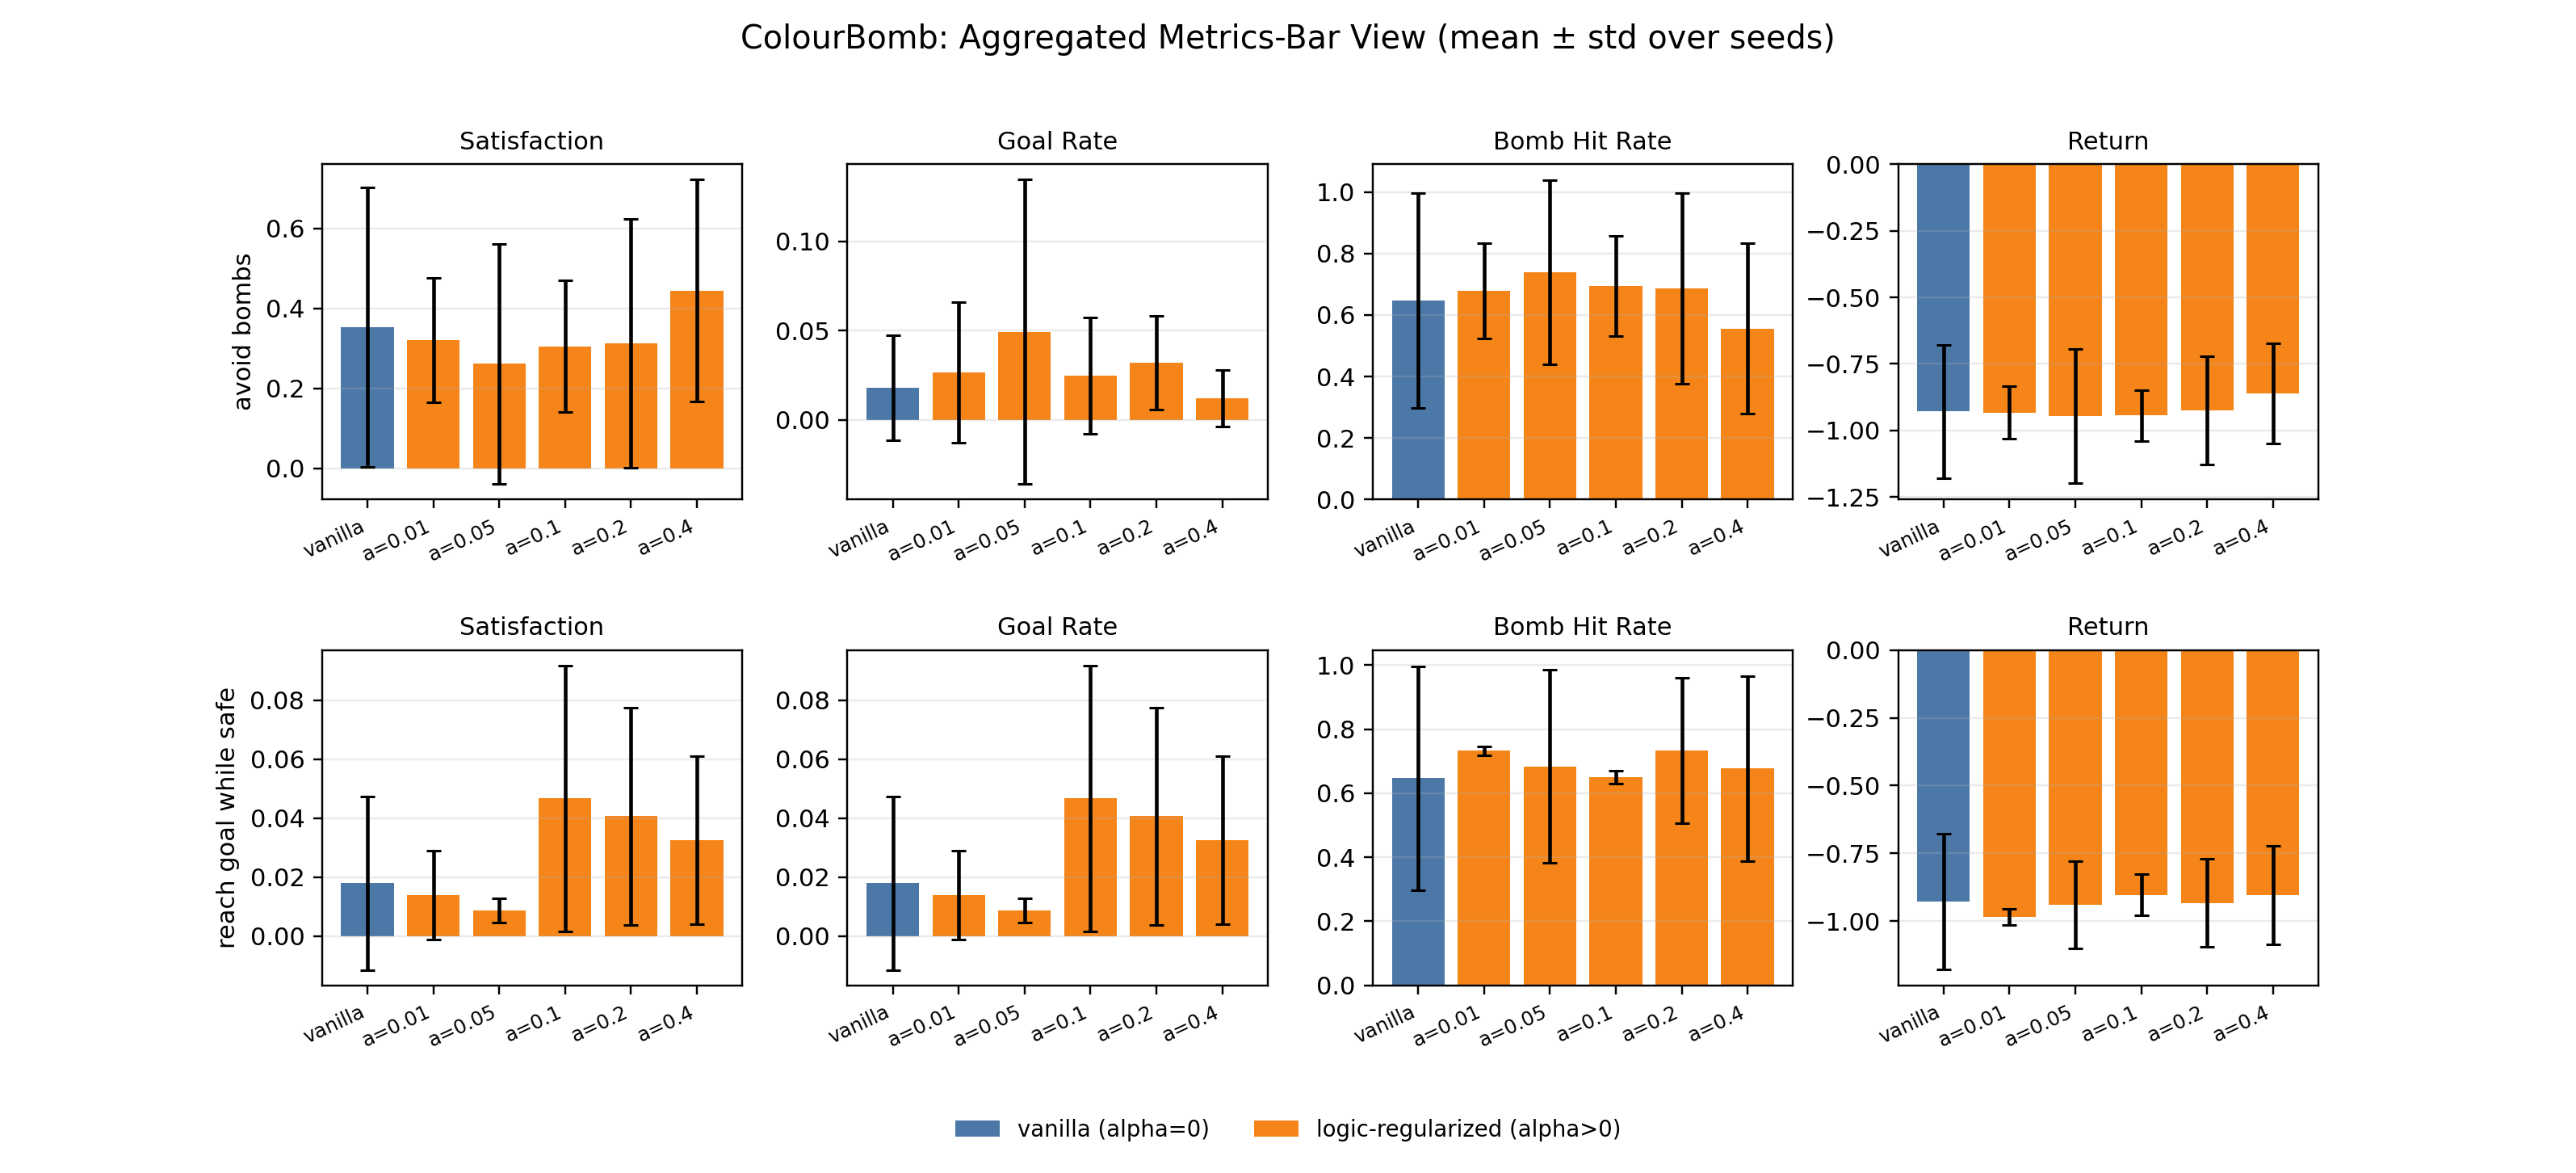
\includegraphics[width=\linewidth]{figures/colourbomb/cb_metrics_bar_example.png}
\caption{Improved metrics-bar style summary (aggregated over seeds) for both CB specs. This figure is the publication-style replacement for per-run \texttt{metrics\_bar} plots.}
\label{fig:cb_metrics_bar_example}
\end{figure}

\subsection{Alpha Sensitivity: Reach-While-Safe (\texttt{reach\_goal\_while\_safe})}
Figure~\ref{fig:cb_alpha_tradeoff} highlights the harder temporal objective. Satisfaction and goal rates are substantially lower than the invariant-only case. The best point in this sweep is around $\alpha=0.1$, but absolute performance remains limited, indicating a difficult goal-safety trade-off in the current CB setup.

\begin{figure}[t]
\centering
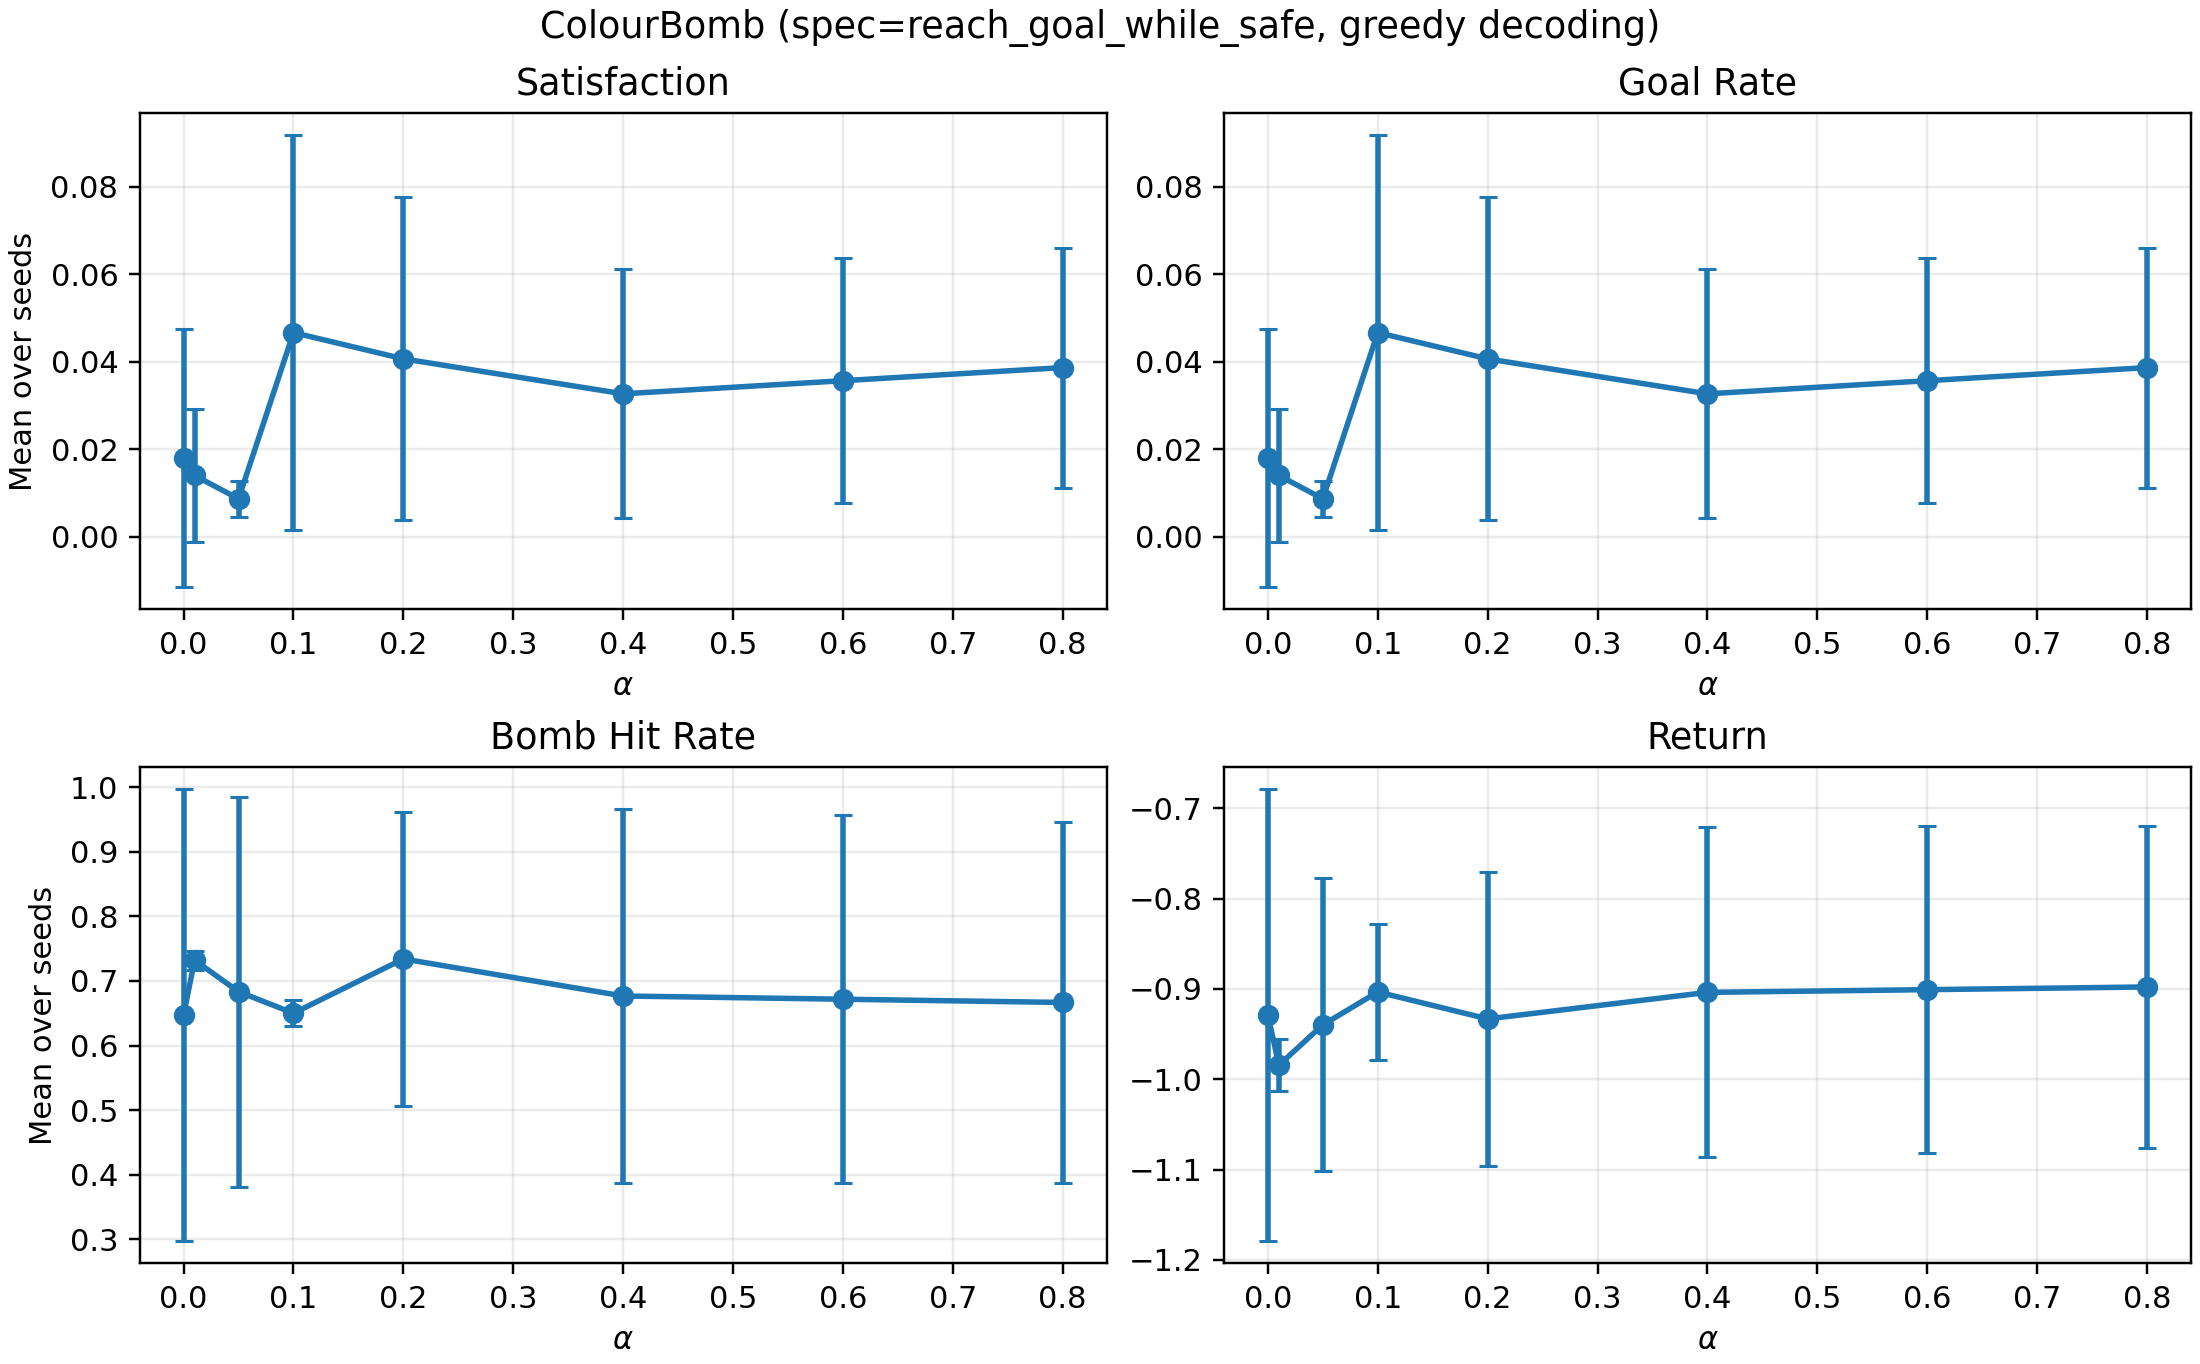
\includegraphics[width=\linewidth]{figures/colourbomb/cb_alpha_sweep_reach_goal_while_safe.png}
\caption{ColourBomb, \texttt{reach\_goal\_while\_safe}, greedy decoding. Mean and std over seeds $\{0,1,2\}$.}
\label{fig:cb_alpha_tradeoff}
\end{figure}

\subsection{Cross-Spec Comparison}
Figure~\ref{fig:cb_cross_spec} compares the best-satisfaction alpha per spec. The invariant objective can be improved mainly by reducing bomb hits, while the reach-while-safe objective remains constrained by low goal attainment.

\begin{figure}[t]
\centering
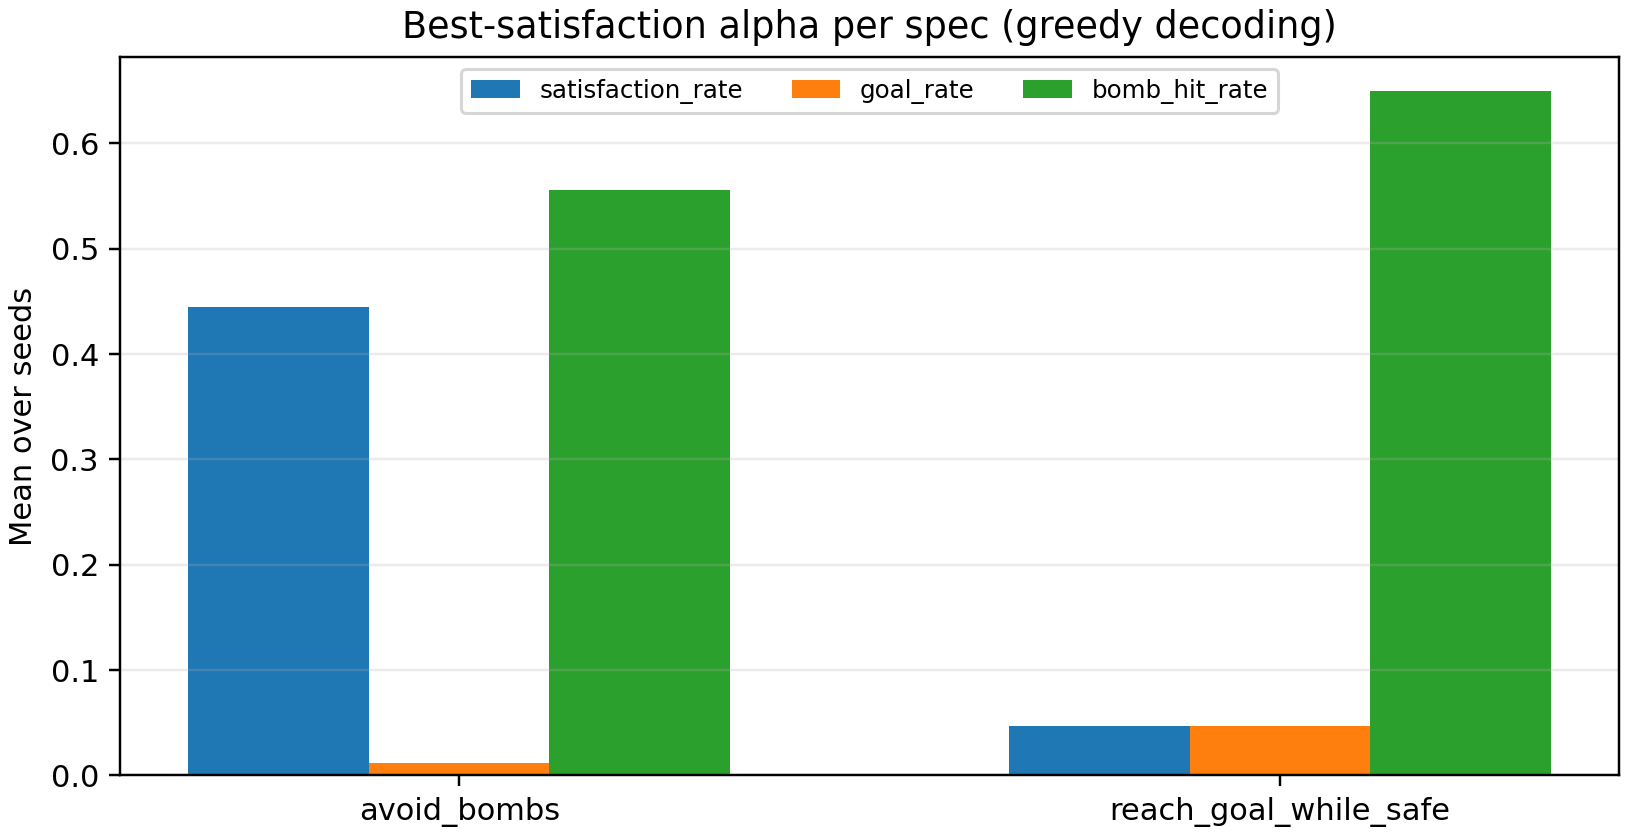
\includegraphics[width=0.9\linewidth]{figures/colourbomb/cb_spec_comparison_goal_vs_safety.png}
\caption{Best-satisfaction alpha per spec (greedy decoding), aggregated over three seeds.}
\label{fig:cb_cross_spec}
\end{figure}

\subsection{Key Quantitative Summary}
Table~\ref{tab:cb_key_results} reports representative operating points from the aggregated CB alpha table.

\begin{table}[t]
\caption{ColourBomb key results (means over seeds 0,1,2; greedy decoding).}
\label{tab:cb_key_results}
\centering
\small
\begin{tabular}{llcccc}
\toprule
Spec & Setting & Satisfaction & Goal & Bomb hit & Return \\
\midrule
\texttt{avoid\_bombs} & vanilla ($\alpha=0$) & 0.353 & 0.018 & 0.647 & -0.929 \\
\texttt{avoid\_bombs} & logic ($\alpha=0.4$) & \textbf{0.445} & 0.012 & \textbf{0.555} & \textbf{-0.862} \\
\texttt{avoid\_bombs} & logic ($\alpha=0.05$) & 0.261 & \textbf{0.049} & 0.739 & -0.946 \\
\midrule
\texttt{reach\_goal\_while\_safe} & vanilla ($\alpha=0$) & 0.018 & 0.018 & 0.647 & -0.929 \\
\texttt{reach\_goal\_while\_safe} & logic ($\alpha=0.1$) & \textbf{0.047} & \textbf{0.047} & 0.650 & \textbf{-0.903} \\
\bottomrule
\end{tabular}
\end{table}

\paragraph{Interpretation.}
The CB experiments support two practical conclusions.
\begin{itemize}
\item Logic regularization can improve safety-oriented metrics, but sensitivity to $\alpha$ is strong and not monotonic.
\item On the harder temporal spec (\texttt{reach\_goal\_while\_safe}), improvements are present but modest; increasing satisfaction currently correlates with only small gains in goal success.
\end{itemize}

\section{Conclusion}

We presented a neurosymbolic framework for injecting \ltlf constraints into transformer-based policies for offline RL. Our approach aims at constructing an automaton-aware decision mechanisms that guide trajectory generation, and it relies on two features: a differentiable representation of DFAs and a differentiable logic loss that regularizes the training objective. 
We appliead the proposed framework to Trajectory Transformers and Decision Transformers. Unlike related popular approaches, we don't need to engineer the underlying reward function, nor we need to focus on a small subset of temporal specifications.
%
Preliminary experiments on the ColourBomb navigation benchmark show that logic regularization can improve constraint satisfaction while maintaining competitive task performance.
These findings suggest that integrating symbolic background knowledge into offline sequence-based RL is a promising direction for improving policy reliability in safety-critical domains. Future work will extend the empirical evaluation to additional benchmarks, model architectures, temporal specifications, and decoding mechanisms. It would be significant also to perform an extensive end-to-end comparison with well-established frameworks for Safe RL.


\begin{credits}

\subsubsection{\ackname} This work has been supported by the the PNRR MUR project FAIR (No. PE0000013), and the Italian National Ph.D. on Artificial Intelligence at Sapienza University of Rome.

\begin{comment}
\subsubsection{\discintname}
It is now necessary to declare any competing interests or to specifically
state that the authors have no competing interests. Please place the
statement with a bold run-in heading in small font size beneath the
(optional) acknowledgments\footnote{If EquinOCS, our proceedings submission
system, is used, then the disclaimer can be provided directly in the system.},
for example: The authors have no competing interests to declare that are
relevant to the content of this article. Or: Author A has received research
grants from Company W. Author B has received a speaker honorarium from
Company X and owns stock in Company Y. Author C is a member of committee Z.
\end{comment}

\subsubsection{\discintname}
The authors have no competing interests to declare that are
relevant to the content of this article.

\end{credits}


%
% ---- Bibliography ----
%
% BibTeX users should specify bibliography style 'splncs04'.
% References will then be sorted and formatted in the correct style.
%
% \bibliographystyle{splncs04}
% \bibliography{mybibliography}
%

\bibliographystyle{splncs04}
\bibliography{bibliography}

\begin{comment}
\begin{thebibliography}{8}
\bibitem{ref_article1}
Author, F.: Article title. Journal \textbf{2}(5), 99--110 (2016)

\bibitem{ref_lncs1}
Author, F., Author, S.: Title of a proceedings paper. In: Editor,
F., Editor, S. (eds.) CONFERENCE 2016, LNCS, vol. 9999, pp. 1--13.
Springer, Heidelberg (2016). \doi{10.10007/1234567890}

\bibitem{ref_book1}
Author, F., Author, S., Author, T.: Book title. 2nd edn. Publisher,
Location (1999)

\bibitem{ref_proc1}
Author, A.-B.: Contribution title. In: 9th International Proceedings
on Proceedings, pp. 1--2. Publisher, Location (2010)

\bibitem{ref_url1}
LNCS Homepage, \url{http://www.springer.com/lncs}, last accessed 2023/10/25
\end{thebibliography}
\end{comment}

\end{document}